%%%%%%%%%%%%%%%%%%%%%%%%%%%%%%%%%%%%%%%%%%%%%%%%%%%%%%%%%%%%%%%%%%%%%%%%%%%%%%%%
%2345678901234567890123456789012345678901234567890123456789012345678901234567890
%        1         2         3         4         5         6         7         8

%\documentclass{article}
\documentclass[letterpaper, 10 pt, conference]{ieeeconf}  % Comment this line out
                                                          % if you need a4paper
%\documentclass[a4paper, 10pt, conference]{ieeeconf}      % Use this line for a4
                                                          % paper


\overrideIEEEmargins
% See the \addtolength command later in the file to balance the column lengths
% on the last page of the document

\usepackage[protrusion=true,expansion=true]{microtype}
\usepackage{cite}
\usepackage{graphicx}
\usepackage{hyperref}
\usepackage{url}
\graphicspath{{figs/}}
\DeclareGraphicsExtensions{.pdf,.jpg,.png}

\usepackage{ifthen}

\usepackage[utf8x]{inputenc}

\usepackage[draft]{fixme}

\usepackage{listings}
\usepackage{alltt}
\usepackage{fancyvrb}


\newcommand{\concept}[1]{{\small \texttt{#1}}}

\newcommand{\stmt}[1]{{\footnotesize \tt $\langle$ #1\relax$\rangle$}}
%\newcommand{\stmt}[1]{{\footnotesize $\langle\stmttt#1\relax\rangle$}}
%\newcommand{\rawstmt}[1]{{\footnotesize \stmttt#1\relax}}
%\def\stmttt#1 #2 #3\relax{
%\texttt{\IfBeginWith{#1}{?}{\textbf{#1}}{#1} \IfBeginWith{#2}{?}{\textbf{#2}}{\emph{#2}} \ifthenelse {\equal{#3}{true} \OR \equal{#3}{false}}{\emph{#3}}{\IfBeginWith{#3}{?}{\textbf{#3}} {#3}}}}

%\newcommand{\setstmt}[1]{{\footnotesize [\setstmttt#1\relax]}}
%\def\setstmttt#1,#2\relax{\stmttt#1\relax, \stmttt#2\relax}


\newcommand{\ie}{{\textit{i.e.\ }}}
\newcommand{\cf}{{\textit{cf\ }}}
\newcommand{\eg}{{\textit{e.g.\ }}}


\title{\LARGE \bf
Explicit Knowledge and the Deliberative Layer: Lessons Learned
}

\author{Séverin Lemaignan and Rachid Alami\\
CNRS-LAAS, 7 av. du Colonel Roche, F-31077 Toulouse, France\\
Université de Toulouse, UPS, INSA, INP, ISAE, LAAS, F-31077 Toulouse, France\\
{\tt surname.name@laas.fr}
}

\begin{document}

\maketitle
\thispagestyle{empty}
\pagestyle{empty}


%%%%%%%%%%%%%%%%%%%%%%%%%%%%%%%%%%%%%%%%%%%%%%%%%%%%%%%%%%%%%%%%%%%%%%%%%%%%%%%%
\begin{abstract}

Over the last four years, we have been slowly ramping up explicit knowledge
representation and manipulation in the deliberative and executive layers of our
robots. Ranging from situation assessment to symbolic task planning, from
verbal interaction to event-driven execution control, we have built up a
\emph{knowledge-oriented} architecture which is now used on a daily basis on our
robots.

This article presents our design choices, the articulations between the diverse
deliberative components of the robot, and the strenghts and weaknesses of this
approach. We show that explicit knowledge management is not only a convenient
tool from the software engineering point of view, but also pushes for a
different, more \emph{semantic} way to address the decision-making issue in
autonomous robots.

\end{abstract}


%%%%%%%%%%%%%%%%%%%%%%%%%%%%%%%%%%%%%%%%%%%%%%%%%%%%%%%%%%%%%%%%%%%%%%%%%%%%%%%%
\section{A Knowledge-Oriented Architecture}

\subsection{Towards the cognitive robot at LAAS}

Natural interaction and cooperation are the current (dare we say,
\emph{short-term}) targets for the human-robot interaction community. They are
keys to the broad class of \emph{interactive manipulation problems}: several
agents agree on a (more or less implicit) joint goal that requires some sort of
cooperation to be successfully achieved. This class of problems involves both
dialogue and manipulation and they are often not completely defined at
start-up: they require iterative and interactive resolution.

Over the last years we have focused our efforts on identifying the cognitive
prerequisites of these challenges, and giving them experimental reality on the
robots: what is required for a sentence like ``Let's dress the table together''
to be understood by the robot, correctly interpreted in the spatial and
temporal context of the interaction, and eventually transformed into a set of
actions?

We have chosen to tackle the challenge from several ends: human-aware
navigation and motion planning (\cite{...Mamoun}), situation assessment coupled
with motion planning (\cite{...}), projection of ``mightabilities'' that
anticipates what surrounding agents may do (\cite{Amit...}), and the design and
deployment of a pervasive \emph{knowledge-centric} software architecture.

We focus in this paper on that last item, to present what that means, and what
are the benefits and drawbacks.

\subsection{Deployment on robots}

While we do not present them here, the ideas and techniques pertaining to this
paper have been all implemented and tested on several robots (see previously
reported experiments in~\cite{Lemaignan2010, Ros2010b, Lemaignan2011a,
Warnier2012a}). Videos presenting some of these experimental results can also
be watched online at~\url{http://www.laas.fr/~slemaign}.

\subsection{Article overview}

We first describe with more details how the deliberative layer of our robots is
built and why this monolithic functional group enables what we call a
\emph{knowledge-oriented} architecture. The first section also introduce our
central knowledge management tool, the ORO server.

The next sections go over each of the facets of this deliberative layer: how
knowledge is produced asynchronously from geometric reasoning, how the robot
conducts grounded multi-modal interaction with humans, how knowledge is used by
decision-making components like the robot controller or the task planner, and
finally, how our knowledge-centric architecture enables the implementation of
specific internal cognitive processes.

We conclude the article with a discussion about the strenghts and weaknesses of
such a knowledge-oriented architecture, fron three perspectives: the architect,
the IA expert and the cognitician.


\section{The LAAS deliberative layer}

\cite{Alami2011}

\begin{figure*}
        \centering
        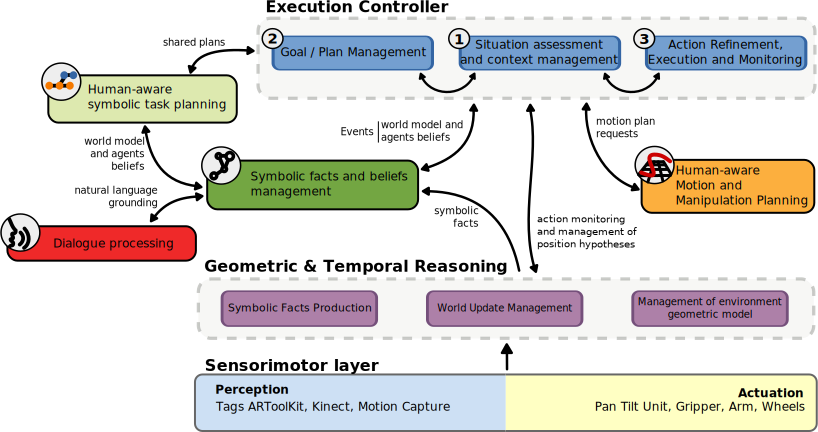
\includegraphics[width=1.7\columnwidth]{archi}
        \caption{Overview of the LAAS deliberative layer.}
        \label{fig|archi}
\end{figure*}



We can give a broader look at the knowledge and the streams of knowledge in our
systems.  Based on the experience gained while developing and deploying {\sc
ORO}, our ontology-based knowledge server, we have presented how symbolic
knowledge could be produced from perception and geometric reasoning in modules
like {\sc SPARK}, a grounded, perspective-aware, geometric reasoner. We have
seen how symbolic knowledge could be reused by different control systems and
task planners like {\sc Cram}, {\sc SHARY}, {\sc pyRobots}, the {\sc CLSU
Toolkit} or {\sc HATP} and how they take advantage of semantic abstractions
provided by knowledge base. We have also presented the bidirectional
integration of {\sc Dialogs}, a natural language processor for English, with
the knowledge base.

Altogether, these components compose an architecture that we call
\emph{knowledge-oriented}:

\begin{itemize}
    
    \item{Knowledge is explicitly stored in one central and consistent
    repository of facts, accessible by all modules.} 

    \item{Knowledge is represented in a strict formalism (OWL statements) and
    with a clearly defined vocabulary (stated in the common-sense ontology).}

    \item{The first two points enable both a loosely-coupled architecture where
    modules can very easily be removed or replaced by other ones as long as
    they share the same semantics (modules are defined by the knowledge they
    produce),} 

    \item{and a \emph{symbolic} reactive, event-driven approach to supervision.
    By managing events at the same level as the reasoner, we take full
    advantage of the inference abilities of ORO to trigger events whose
    \texttt{true} conditions can be inferred.} 

    \item{Finally, this architecture allows for the combination of very
    different knowledge modalities in a single homogeneous environment,
    bringing mutual benefits to components. For instance, the dialogue
    processing module can perfectly run without any geometric
    perception, but its disambiguation routines can transparently
    benefit from it when available (since richer symbolic descriptions of
    objects are then available).}

\end{itemize}

This architecture moves away from standard layered approaches. Interactions
between components are mostly bidirectional and, from the software components
point of view, we do not introduce layers of abstraction (we do, however, have
access to the lower level modules of the robot to execute actions, but all
cognition-related modules reside at the same level). This is especially visible
for the dialogue input processing. This component does not simply act as an
alternative perceptual input to the symbolic database, but also actively
queries previously acquired knowledge to disambiguate and validate the newly
created symbolic knowledge.

Our architecture relates but is to be distinguished from \emph{Beliefs,
Desires, Intentions} (BDI) architectures. BDI architectures are primarily
focused on \emph{practical reasoning}, \ie the process of deciding, step by
step, which action to perform to reach a goal (as summarised by
Woolridge~\cite{Woolridge1999}). The management of the interaction between
knowledge (the beliefs) and task and plan representation and execution (the
desires and the intentions) is central, and aims at selecting at each step the
best subgoal. It becomes then an intention that the robot commits to.

This interaction between knowledge and actions is also central to our approach
(as for any cognitive system), but task representation and task execution is
not seen as a monolithic, central function: it is one of the activities of the
robot, actually split between communication components (that can acquire
desires from interaction with agents, amongst other things) and an execution
controller that may decide to take an incoming desire into account to create
its own internal goals. The controller generates and controls intentions from
these goals with the help of a symbolic task planner, that has also direct
access to the knowledge base.

The architecture is not only focused on this workload, and other
activities are conducted without being explicitly considered as desires:
assessment of the situation and the environment, dialogue (including
performative dialogue that can possibly change the internal state of the robot,
but does not lead to the creation of desires,  like question answering or
statement assertion), various background monitoring and recognition tasks, etc.

Regarding the anchoring question, this architecture is bidirectional. The
components we described provide a \textit{bottom-up} grounding process: SPARK
and \textsc{Dialogs} constantly build and push new symbolic contents about the
world to ORO where it becomes accessible to decisional layers. In parallel, ORO
relies on reasoning in a \textit{top-down} way to produce new facts that may
trigger in return physical behaviours. 

We believe that this \emph{knowledge-oriented} approach has a strong potential
not only to enable rich human-robot interaction, but also as a broader approach
to information alignment and fusion in complex robotic systems.  The
versatility of this paradigm could be illustrated by a simple imaginary
scenario with a blind robot and a deaf robot. The blind robot does not see (no
cameras or alike), but someone can verbally describe a scene to it. On the
other hand, the deaf robot has a good vision system, but cannot process verbal
input.  Without any changes to the software architecture that we described,
control modules of both robots could equally perform the same tasks since all
the knowledge is abstracted and centralised (note that to actually implement
this imaginary situation, the blind robot would of course need \textit{a
priori} 3D models of objects talked about to enable planning or pick and place
actions, and the deaf robot would require at least some gesture interpretation
to understand orders).

This architecture may also contribute to bring closer robotics and psychology:
it provides clear entry points to implement some classical psychology tests to
robots. For instance, we presented experiments focused on issues related to
perspective taking. By explicitly enabling independent modeling of the beliefs
of each agent, our architecture is especially well suited to set up cognitive
and psychological experiments that involve a theory of mind, such as
\emph{False-Belief} experiments, as recently presented in~\cite{Warnier2012a}.

\subsection{Knowledge Model}

\cite{Lemaignan2010}

%%%%%%%%%%%%%%%%%%%%%%%%%%%%%%%%%%%%%%%%%%%%%%%%%%%%%%%%%%%%%%%%%%%%%%%%%%%%%%%%
\section{Situation Assessment}
\label{sect|sit-ass}

\begin{figure}
        \centering
        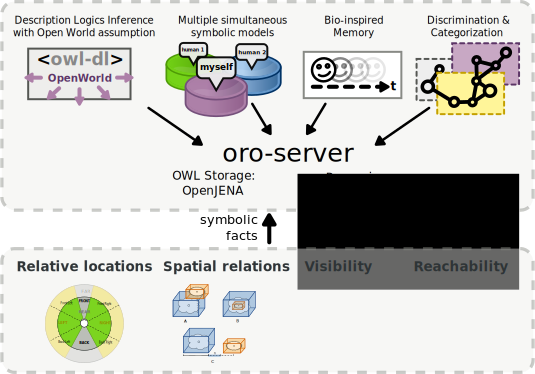
\includegraphics[width=\columnwidth]{spark-oro}
        \caption{Functional overview of knowledge base (\emph{oro-server}, top part) and the geometric situation assessment module (\emph{SPARK}, bottom part)}
        \label{fig|spark-oro}
\end{figure}

\cite{Sisbot2011}

%%%%%%%%%%%%%%%%%%%%%%%%%%%%%%%%%%%%%%%%%%%%%%%%%%%%%%%%%%%%%%%%%%%%%%%%%%%%%%%%
\section{Communication}
\label{sect|com}

\subsection{Natural language grounding}

One of the field of human-robot interaction where the introduction of the
semantic layer has been most beneficial is natural language processing.
\cite{Lemaignan2011a} details the techniques and the tool called
\texttt{dialogs} that we have developed for English language parsing and
grounding, for (minimalist) dialogue management and for verbalisation.

Natural language input (in experiments, we rely on an Android-based interface
running on a tablet, with Google-based speech recognition, for the input) is
parsed into a grammatical structure, and each sentence atoms are resolved with
the help of the ontology to ground classes (when a user says ``pick the can'',
to which instance of \emph{can} the user refers to?) and actions. Sentences are
sorted into questions, desires and statements, and processed accordingly.

The system supports quantification (``give me \{a|the|some|all|any|...\} can''),
thematic roles attached to actions, interactive disambiguation (the robot asks
questions when needed), anaphora resolution (``give \emph{it} to me'') based on
dialogue history. It also permits knowledge extension by learning new semantic
structures (for instance, a sentence like ``learn that cats are animals'' is
converted into \stmt{Cat subClassOf Animal}, even if \concept{Cat} is not known
beforehand) and tries to translate \emph{states} (``I'm tired'') into
\emph{experiences} (\stmt{HUMAN experiences state\_1, state\_1 hasFeature
tired}).

\subsection{Disambiguation at semantic level}

One prototypical example of semantic disambiguation has been given in
\cite{Ros2010b} with the child's \emph{spygame}: two players are facing
each other with a set of random objects in-between, one player mentally choose
one object, and the other player has to guess the object by asking closed
questions like \emph{Is your object small or large?}. Based on the knowledge it
has acquired, the robot is able to minimize the number of questions required to
find the object.

When playing this kind of game, however, the issue arises that the robot has no
way to select which knowledge about the object is relevant in the interaction
context. For instance, the knowledge base may store facts like \stmt{obj1 type
ActiveConcept} (which internally means that this concept was mentioned in a
discussion in the last few seconds): this information is not a relevant
property of \concept{obj1} when trying to disambiguate concepts with humans.
This distinction between \emph{internal knowledge} (meaningful to
the systme only) and \emph{common knowledge} (whose meaning is understood by
all the interactors) has not been properly dealt with in our architecture.

Besides, even knowledge that belongs to what we call \emph{common knowledge},
may not be appropriate in a given interaction context. For instance, the system
may compute that at a given instant, the human is looking at the object:
\stmt{human looksAt obj1}. This property makes sense to both parties, but in
the context of the \emph{spygame}, we would like to mainly use immanent
properties, not volatile like a gaze. More research is required to precise this
idea of contexts and knowledge class attached to them.


\fxnote{Mention failures like 'placeOing'}

\subsection{Multi-modal communication}

Because the main communication channel between component is semantic data,
different communication modalities (explicit like verbal, dectic or based on
gaze, or implicit like postures) are accessed in an homogeneous way.

The grounding process copes with and integrates the different physical
modalities at two disctint levels.

First, the grounding module explicitely check for the presence and value of
particular facts: for instance, when a set of instances match a category (the
human says ``give me the bottle'' and the robot knows about three bottles), the
module may decide (it actually depends on the quantifier preceding the class:
\emph{the}, \emph{a}, \emph{any}...) to discard some of them based on their
\emph{visibility} by the speaker (implicit communication context built from the
human posture).

Another example, when the human says ``this'', the robot checks if the human is
currently both pointing and looking at some object. In that case, \emph{this}
is replaced by the object focused on.

Note that, while the system benefits from the complementary modalities, they
are not required. The dialogue system would work as well in a purely verbal
setting.

The second level of integration of multi-modality is implicit: by computing
symbolic properties from the geometry, richer descriptions and hence
discrimination possibilities are available: for instance, if reachability is
available, the robot may asks ``do you mean the bottle that is accessible to
me?'' to discriminate between the three bottles. That way, procedures relying
on discrimination transparently benefit from added modalities.

%%%%%%%%%%%%%%%%%%%%%%%%%%%%%%%%%%%%%%%%%%%%%%%%%%%%%%%%%%%%%%%%%%%%%%%%%%%%%%%%
\section{Robot Control}
\label{sect|ctrl}

\subsection{Modeling the knowledge related to the interaction}

We split the interaction situations stemming from the situation assessment and
communication components in two categories: \emph{desires} and
\emph{experiences}.

Experiences comprise of emotions and questions

\subsection{Task planning}

In order to devise how a given goal can be accomplished, the robot has to
elaborate a plan,\ie a set of actions to be achieved by the robot and its human
partners.  We use in our architecture the HATP planner~\cite{Alili2009} (for
Human Aware Task Planner).  HATP is based on a Hierarchical Task Network (HTN)
refinement, which performs an iterative task decomposition into sub-tasks until
reaching atomic actions.  The planning domain defines a set of methods
describing how to decompose a task and can be seen as the procedural knowledge
of the robot.

In order to produce a collaborative behaviour, the robot plans not only for
itself but also for the other agents. The planning domain of each agent is
instantiated from the agent-specific model in the ORO server. The resulting
plan, called ``shared plan'' is a set of actions that form a stream for each
agent involved in the goal achievement. HATP can also be tuned by setting up
different costs depending on the actions to apply and by taking into account a
set of constraints called \emph{social rules}. This tuning aims at adapting the
robot's behaviour according to the desired level of cooperation of the robot.


Two important remarks: because HATP is a generic symbolic task planner, we have
been able to design a planning domain at a semantic level which is close to the
one used in the human-robot dialogue (the planner vocabulary contains concepts
like \texttt{give}, \texttt{table}, \texttt{is on}...). Hence only a few
ontology rules have been required to map both the knowledge extracted from the
situation assessment and the statements originated from the verbal interaction
to the planner domain.

Second remark, after some research (see appendix B of~\cite{ma these} for a
detailled discussion)  we have decided not to represent neither tasks nor plans
in the ontology: the planning domain (with tasks pre- and postconditions) is
stored in a specific format, outside of the knowledge repository, and the
resulting plans are directly communicated to the robot controller. The ontology
formalism that we have adopted (namely OWL) does not appear to be a satisfaying
reprepresentation language for concepts that are both tightly bound to time
representation and non-monotonic. Other researches (\cite{tenorth...}) have attempted with more success (\fixme{regarder ca!!}).

%%%%%%%%%%%%%%%%%%%%%%%%%%%%%%%%%%%%%%%%%%%%%%%%%%%%%%%%%%%%%%%%%%%%%%%%%%%%%%%%
\section{Internal Cognitive Processes}
\label{sect|intern}

\subsection{Theory of Mind}

\cite{Warnier2012a}

\subsection{Working Memory}

%%%%%%%%%%%%%%%%%%%%%%%%%%%%%%%%%%%%%%%%%%%%%%%%%%%%%%%%%%%%%%%%%%%%%%%%%%%%%%%%
\section{Conclusions}
\label{sect|conclusion}

We conclude this article with three different perspectives on the knowledge-centric
techniques we have presented here: first, the \emph{architect perspective}:
what are the pro and cons of our approach from an engineer point of view. Then,
the \emph{logician perspective}: does the promise of automated reasoning for
robots really comes to fruition with ontologies? And eventually the
\emph{cognitician perspective} or how explicit knowledge manipulation endows
our robots with new cognitive capabilities.

\subsection{The Architect view: loose coupling and modalities merging}

In this article, we have presented several sub-systems of our robots: a module for geometric
reasoning and situation assessment (written in C++), a natural
language interface (written in Python), a symbolic task planner (written in
C++), two execution controller (one written in Python, one in PRS). These
modules communicate together through RDF statements with only a few exceptions.

Since these statements are anchored in the robot's pool of knowledge, they
actually convey \emph{meaning} through the system (for instance, when the
dialog module or the task planner or the execution controller uses the symbol
{\tt Give} \emph{means}, it refers to the abstract class of all give actions, which are also stated
to be a kind of purposeful actions). This has one important consequence from
the perspective of the system architecture: modules interfaces are only defined
in term of knowledge consumption and/or production. This brings good decoupling
properties. For instance, the output of the dialog module is a new
\emph{situation desired} by the speaker. This module can be transparently
replaced or completed by any other module that produces the same chuncks of
knowledge. Only a thin protocol layer remains to get the modules to interact
together. This allows us to implement (otherwise difficult) merging of
radically different perception modalities like vision (the robot sees an object on
a table) and verbal description (a human says to the robot another object is
under the table): both are converted to RDF statements ({\tt obj1 type Object},
{\tt obj1 isOn table1} and {\tt obj2 type Object}, {\tt obj2 isUnder table1})
and made available to the other robot modules.

Another consequence is that the communication channels are {\it
defacto} defined by the semantics of the information they
convey. This allows the system designers to think in term of which module
produces or needs which knowledge, instead of which module produces which
service. We found this approach to be very helpful when implementing cognitive
functions like the theory of mind, the perspective taking or the natural
language grounding.

Lastly, another good property of knowledge-based communication between module
is the \emph{cognitive observability} of the system: by logging queries between
modules (which is even easier in our case since we rely on a central knowledge
management), one can trace the interactions between the robot systems at a high
abstraction level. We will come back below on the significance of this property
from the cognitive point of view.

The knowledge-centric architecture also has downsides. We can name here a few.

Because the sources of knowledge the robot has to deal with are multiple and
often not known at startup (typically, the knowledge generated by a verbal
interaction with a human), it is difficult to formally guarantee reliability.

Also, it must be noted that actuation itself is directly piloted by the
execution controller through standard RPC calls (ROS actions and/or Pocolibs
requests): no knowledge abstraction takes place.

And obviously, many aspects like uncertainty management, modal logics,
non-monotonic reasoning,... remain to be explored to gain the level of
expressiveness required to cover many of the more complex human-robot
interaction scenarii.

\subsection{The Logician view: the importance of trivial inferences}

\begin{quote}

    Where to find milk? Milk is a subclass of dairy which is itself a subclass
    of a perishable goods. The usual storage place for perishable goods is the
    fridge, so the milk is likely to be found in a fridge.

\end{quote}

This example of reasoning, quoted from Moritz Tenorth, is a good example of
simple yet non-trivial reasoning. As a matter of fact, only very few of such
reasoning cases where positively identified in our scenarii and experiments
(and consequently implemented as rules in ORO).

The design choices of our architecture partially explain that fact: first, the
planning task (which is the prototypical reasoning task) is delegated to a
dedicated, external planner. Then, time is not represented in ORO, and
consequently no temporal reasoning takes place at this level: action
recognition or monitoring are handled by other layers, and the underlying
reasoning tasks are not implemented as explicit symbolic rules in the knowledge
base.

The experiments we have conducted are also likely to have too simplistic
semantics to let complex reasoning needs to emerge. Scenarii with more complex
semantics would be desirable to better stress the expressiveness and inference
abilities provided by description logics.

Is reasoning at the knowledge level immature or even superfluous, then? Not so:
hundreds of trivial (from a human point of view) inferences are continuously
produced by the system (translating inheritance relations, domain/range
constraints, transitivity, etc.) and encode a large amount of common-sense
knowledge that would be tedious, to say the least, to manually assert. These
trivial inferences are all the more important that an expressive knowledge
representation language is used: when a language like OWL allows to directly
represent high-level concepts like partitions, cardinality restrictions,
properties' ranges and domains, it leads to a more implicit (because more
abstract) description of the vocabulary that in turn requires more underlying
reasoning. With the progress in the understanding of the relations between
expressiveness and (tractable) satisfiability, along with the progress of
reasoners, more and more of the inferences do not need to be explicit anymore,
and consequently move behind the scenes.

And we predict that \emph{common-sense encoding} is likely to remain the main
application of reasoning in our robotic architectures, where reasoning related
to decision making mostly happen outside the knowledge representation system.


\subsection{The Cognician view: palpable knowledge and semantic thinking}

The main motive goal was to transform the knowledge in the robot from some ubiquitous,
pervasive, multi-modal and, most importantly, mostly undefined feature of the
system into an observable, quantifiable, manipulable resource, what we could
call a \emph{palpable} feature.

This transformation, both from the technical point of view (the ORO server, the
ontologies, the bindings, etc.), and as a more subtle change in the practises
related to the development of robotic components, is the main contribution of
this thesis.

Knowledge is not an abstract concept anymore: it is a set of statements, in
most cases directly intelligible to the developers, stored in one place. We can
export them, monitor them, review them, question them.

Communication between the robot's module is now conceived in term of what are
the \emph{semantics} of the information flows, instead of a simple
compatibility of interfaces. When defining the frontiers of a robotic
component, we do not think anymore only in term of ``is the interface complete
and self-contained'', but also in term of ``is the semantic complete and
consistent?''. This allow a deeper, more correct modularity: two modules that
share the same, well-defined semantic can be confidently exchanged. When we
remove or disable a component (the dialogue processing, the geometric
reasoning, ...), we know precisely what knowledge will not be available
anymore.

We call this new property of our robot, that allows for both qualitative and
quantitative analysis of the beliefs, its \emph{cognitive observability}.

It is somewhat related to the idea of \emph{cognitive penetrability} introduced
by Pylyshyn~\cite{Pylyshyn1989} in 1989, in the context of the study of
possible strong equivalences between computational models and the
\emph{psychological reality}:

\begin{quote}

    [One of the criterion] relies on the assumption that we can identify
    certain clear cases of phenomenon that should be accounted for at the
    knowledge level, that is, in terms of the representations alone, rather
    than in terms of properties of the cognitive architecture. Phenomena that
    depend in a rational way on subjects' goals, beliefs, and utilities are a
    case in point. For example in psychophysics we assume that if a measure
    (such as a threshold) changes systematically as we change the payoffs (that
    is, the relative cost of errors of commission and of omission), then the
    explanation of that change must be given at the knowledge level -- in terms
    of decision theory -- rather than in terms of properties of sensors or
    other mechanisms that are part of the architecture. In general showing that
    certain empirical phenomena are sensitive to goals and beliefs (or what I
    call \emph{cognitively penetrable}) is prima facie evidence that they
    should not be attributed to properties of the architecture.

\end{quote}

The introduction of an explicit \emph{knowledge level} in our architecture
makes it possible to effectively assess the cognitive penetrability of the
whole robot behaviours (this is however not new, and traditional BDI
architectures would also make this claim).

\section*{Acknowledgment}

This work has been supported by EU FP7 ``SAPHARI'' under grant agreement no. ICT-287513.

\bibliographystyle{IEEEtran}
\bibliography{IEEEabrv,biblio}


\end{document}
